\section{Reparameterisation of the Schwarzschild Solution}

In this section the Kasner solution of the vacuum field equations is derived from the Schwarzschild solution by taking the limit as the mass goes to infinity. It is then shown that the special case of the Kasner solution with no mass is equivalent to a novel form of Minkowskian space-time. (what do we want the Kasner vacuum solution for???). Start with the Schwarzschild Solution of the vacuum field equations given by

\begin{equation}\label{Schwarz_Sol} 
\epsilon {\mathrm{d}s}^2 = {\left(1 - \frac{2m}{r}\right)}^{-1} {\mathrm{d}r}^{2} + r^2 ({\mathrm{d}\theta}^2 + {{\sin}^2 \theta}{\mathrm{d} \phi}^2) - \left(1 - \frac{2m}{r}\right) {\mathrm{d}t}^2.
\end{equation}

\subsection{Eddington-Finkelstein Coordinate Transformation}

\noindent First, make the Eddington-Finkelstein coordinate transformation

\begin{equation}\label{Ed-Fin_trans}
u = t - r - 2m \ln(r - 2m).
\end{equation}

\noindent Calculate the differentials

\begin{align*}
\mathrm{d}u & = \mathrm{d}t - \mathrm{d}r - \frac{2m \mathrm{d}r}{r - 2m},\\
            & = \mathrm{d}t - \mathrm{d}r{\left( 1-\frac{2m}{r}  \right)}^{-1},\\
\mathrm{d}t & = \mathrm{d}u + {\left( 1-\frac{2m}{r}  \right)}^{-1} \mathrm{d}r, 
\end{align*}

\noindent and sub them into Eqn.(\ref{Schwarz_Sol}).

\begin{equation*}
\epsilon {\mathrm{d}s}^{2} = {\left( 1-\frac{2m}{r}  \right)}^{-1} \mathrm{d}r^2 + r^2 ({\mathrm{d}\theta}^2 + {{\sin}^2 \theta}{\mathrm{d} \phi}^2) - {\left( 1-\frac{2m}{r}  \right)} {\left( \mathrm{d}u + {\left( 1-\frac{2m}{r}  \right)}^{-1} \mathrm{d}r \right)}^{2},
\end{equation*}

\noindent which gives the result,

\begin{equation}\label{Reparameterisation_Schwarzschild_Before_Limit}
\epsilon {\mathrm{d}s}^{2} = r^2 ({\mathrm{d}\theta}^2 + {{\sin}^2 \theta}{\mathrm{d} \phi}^2) - 2 \mathrm{d}u \mathrm{d}r - {\mathrm{d}u}^{2} + \frac{2m}{r} {\mathrm{d}u}^{2}. 
\end{equation}

Note that if $m = 0$ the space-time becomes Minkowskian, as expected. If $r = 0$ in this Minkowskian space-time the line element becomes

$$ \epsilon {\mathrm{d}s}^2 = - {\mathrm{d}u}^{2},$$

\noindent which implies that $\epsilon = -1$ and the first integral of this trajectory is also equal to $-1$. Thus $r = 0$ is a time-like world-line in Minkowskian space-time, with proper time u.(ERROR CHECK ITS A GEODESIC???NEED TO CHECK ANSWER WITH HOGAN)

The limit of the Schwarzschild solution as $m \rightarrow \infty$ must be calculated to find the Kasner solution. In its current form the limit cannot be taken, so two suitable coordinate transformations must be made to get it in a more useful form. First Set 

\begin{gather*} 
u = \mu u', \\
r = {\mu}^{-1} r',   
\end{gather*} 

\noindent where $\mu = \text{ const}$ so that
  
\begin{gather*} 
\mathrm{d}u = \mu \mathrm{d}u', \\
\mathrm{d}r = {\mu}^{-1} \mathrm{d}r'. \\
\end{gather*} 

\noindent The product of the differentials is then invariant

\begin{equation*}
{\mathrm{d}u}{\mathrm{d}r} = {\mathrm{d}u'}{\mathrm{d}r'}. 
\end{equation*}

\noindent When the new coordinates are subbed into Eqn.(\ref{Reparameterisation_Schwarzschild_Before_Limit}) the Schwarzschild solution becomes

\begin{equation}\label{Reparameterise_Schwarzschild_Next_Before_Limit}
\epsilon {\mathrm{d}s}^2 = {r'}^2 \sin^2 \theta \left\{ \frac{{\mathrm{d}\theta}^2}{\mu^2 \sin^2 \theta} +  \mu^{-2} {\mathrm{d} \phi}^2 \right\} - 2 {\mathrm{d}u'} {\mathrm{d}r'} - \left( \mu^2 - \frac{2 m \mu^3}{r'}\right) {\mathrm{d}u'}^2 . 
\end{equation}

\noindent Now set $m \mu^{3} = k$ or $ m = k \mu^{-3}$ and make another transformation first done by Ivor Robinson(check this???) given by

\begin{align*} 
\sin{\theta} = \frac{1}{\cosh{(\mu \xi)}}, & \mu^{-1} \phi = \eta.  
\end{align*} 

\noindent The second of these transformations gives simply $\mu^{-2} \mathrm{d}\phi^2 = \mathrm{d} \eta^2$. To rewrite the first coordinate transformation, first differentiate.

\begin{align*} 
\cos{\theta} \mathrm{d} \theta & = \frac{-1}{(\cosh(\mu \xi))^{2}} \sinh(\mu \xi) \mu \mathrm{d} \xi, \\
                      & = -{\sin}^{2}\theta \sinh(\mu \xi) \mu \mathrm{d} \xi.
\end{align*}

\noindent Use the forumla $\cosh^2 A - \sinh^2 A = 1$, divide by $\mathrm{d} \xi$ and simplfy using trigonometric identities

\begin{align*}
\cos{\theta} \frac{\mathrm{d} \theta}{\mathrm{d} \xi} & = -\mu \sin^2 \theta \sqrt{\frac{1}{\sin^2 \theta} - 1}, \\
                                    & = - \mu \sin \theta \cos \theta.
\end{align*}

\noindent Finally rewrite in terms of $\mathrm{d} \xi$

\begin{equation*}
\mathrm{d} \xi^2 = {\left( \frac{\mathrm{d} \theta}{\mu \sin \theta}  \right)}^2.
\end{equation*}

\noindent Subbing these transformations into Eqn.(\ref{Reparameterise_Schwarzschild_Next_Before_Limit}) gives

\begin{equation*}
\epsilon {\mathrm{d}s}^2 = \frac{r^2}{\cosh^{2}{\mu \xi}} ({\mathrm{d}\xi}^2 + {\mathrm{d}\eta}^2) - 2 {\mathrm{d}u}{\mathrm{d}r} - \left( \mu^{2} - \frac{2k}{r} \right) {\mathrm{d}u}^2,
\end{equation*}

\noindent where the primes have been dropped for convenience. 

\subsection{The Kasner Solution}

This is now in an appropriate form to take the limit $m \rightarrow \infty$ which is equivalent to $\mu \rightarrow 0$, to obtain

\begin{equation}\label{Kasner_after_limit}
\epsilon {\mathrm{d}s}^2 = r^2 ({\mathrm{d}\xi}^2 + {\mathrm{d}\eta}^2) - 2 {\mathrm{d}u}{\mathrm{d}r} - \frac{2k}{r} {\mathrm{d}u}^2
\end{equation}

\noindent This is still a solution of the field equations but it is no longer the Schwarzschild solution. In this section it is shown to be the Kasner Solution(READ UP ABOUT THIS), which by definition is given by

\begin{equation}\label{Reparameterise_Definition_Of_Kasner} 
\epsilon {\mathrm{d}s}^2 = T^{2p} {\mathrm{d}X}^2 + T^{2q} \mathrm{d}Y^2 + T^{2r} \mathrm{d}Z^2 - \mathrm{d}T^2,
\end{equation}

\noindent such that

\begin{eqnarray*}
p + q + r = 1 = p^2 + q^2 + r^2.
\end{eqnarray*}

To write Eqn.(\ref{Kasner_after_limit}) in this form first make the transformation

\begin{gather*} 
\xi' = \lambda^{-1} \xi, \text{    }  \eta' = \lambda^{-1} \eta, \\
r' = \lambda r,          \text{    }  u' = \lambda^{-1} u,
\end{gather*}

\noindent with $\lambda \vcentcolon = k^{-1/3}$. Subbing in these new coordinates gives

\begin{equation*}  
\epsilon \mathrm{d} s^2 = {r'}^2 (\mathrm{d} {\xi'}^2 + \mathrm{d} {\eta'}^2) - 2 \mathrm{d} u' \mathrm{d} r' + \frac{2}{r'}\mathrm{d} {u'}^2.
\end{equation*}

\noindent Now add and subtract $(r'/2) \mathrm{d} {r'}^2$ to complete the square as follows

\begin{equation*}  
\epsilon \mathrm{d} s^2 = r^2 (\mathrm{d} \xi^2 + \mathrm{d} \eta^2) + \frac{2}{r}{\left( \mathrm{d} u  - \frac{r}{2} \mathrm{d} r\right)}^2 - \frac{r}{2}\mathrm{d} r^2,
\end{equation*}

\noindent where the primes have again been dropped for convenience. Now set

\begin{equation*}
\bar{X} = u - \frac{r^2}{4},
\end{equation*}

\noindent so the differential of $\bar{X}$ is

\begin{equation*}
\mathrm{d} \bar{X} = \mathrm{d} u - \frac{r}{2} \mathrm{d}r,
\end{equation*}

\noindent and the line element can be rewritten in terms of $\bar{X}$,

\begin{equation*}
\epsilon \mathrm{d} s^2 = r^2 (\mathrm{d} \xi^2 + \mathrm{d} \eta^2) + \frac{2}{r} \mathrm{d} \bar{X}^2 - {\left( \frac{r^{1/2}}{\sqrt{2}} \mathrm{d} r\right)}^{2}.
\end{equation*}

\noindent Now define $T$ such that

\begin{equation*}
T = \frac{\sqrt{2}}{3} r^{3/2} \text{,       and    } r = {\left( \frac{3}{\sqrt{2}} \right)}^{2/3} T^{2/3},
\end{equation*}

\noindent which results in the new line element

\begin{equation*}
\epsilon \mathrm{d} s^2 = \left( \frac{3}{\sqrt{2}} \right)^{4/3} T^{4/3} (\mathrm{d} \xi^2 + \mathrm{d} \eta^2) + 2 \left( \frac{\sqrt{2}}{3}\right)^{2/3} T^{-2/3} \mathrm{d} \bar{X}^2 - \mathrm{d} T^2.
\end{equation*}

\noindent Then a final coordinate transformation can be made to remove the unwanted constants, given by

\begin{align*} 
X & = \left[ 2\left( \frac{\sqrt{2}}{3}\right)\right]^{1/2} \bar{X}, \\
Y & = \left( \frac{3}{\sqrt{2}} \right)^{2/3} \xi, \\
Z & = \left( \frac{3}{\sqrt{2}} \right)^{2/3} \eta, \\
\end{align*} 

\noindent to obtain

\begin{equation}\label{Our_Kasner} 
\epsilon {\mathrm{d}s}^2 = T^{-2/3} {\mathrm{d}X}^2 + T^{4/3} \left( \mathrm{d}Y^2 + \mathrm{d}Z^2 \right) - \mathrm{d}T^2.
\end{equation}

\noindent Comparing this result to the general form of the Kasner solution in Eqn.(\ref{Reparameterise_Definition_Of_Kasner}) it is clear that they have the same form with $p=-1/3$ and $q=r=2/3$. Thus the solution obtained by taking the limit of the Schwarzschild solution as $m \rightarrow \infty$ is indeed the Kasner Solution. 

\subsection{Line Element of Minkowskian Space-Time}

Minkowskian space-time reemerges again by setting $k = 0$ in Eqn.(\ref{Kasner_after_limit}), which is equivalent to $m = 0$. 

\begin{equation}\label{Kasner_after_limit_no_k}
\epsilon {\mathrm{d}s}^2 = r^2 ({\mathrm{d}\xi}^2 + {\mathrm{d}\eta}^2) - 2 {\mathrm{d}u}{\mathrm{d}r}
\end{equation}

\noindent Setting $r = 0$ gives $\epsilon {\mathrm{d}s}^2 = 0$. In this section it is demonstrated that $r = 0$ is a null geodesic with $u$ an affine parameter along it and that Eqn.(\ref{Kasner_after_limit_no_k}) is indeed the Minkowskian space-time line element. To verify these properties first let $x^i = (x,y,z,t)$ be rectangular Cartesian coordinates with time in Minkowskian space-time with the usual line element

\begin{equation*} 
\epsilon {\mathrm{d}s_0}^2 = {\mathrm{d}x}^2 + {\mathrm{d}y}^2 + {\mathrm{d}z}^2 - {\mathrm{d}t}^2.
\end{equation*} 

\noindent We note that the trajectory $C$  defined by $x = 0$, $y = 0$, $z = t$ is a null geodesic as it will lie on the light cone of Minkowskian space-time. If $C$ is writen parametrically as $x^i = w^i (u)$ such that $w^i = (0,0,u,u)$ then $u$ is an affine parameter along it. The tangent to $C$ is then computed as

\begin{equation*} 
v^i (u) = \frac{\mathrm{d} w^i}{\mathrm{d}u} = (0,0,1,1).
\end{equation*} 

\noindent As $C$ is a null geodesic the first integral will be $v_i v^i = 0$ and thus $v_i = (0,0,1,-1)$ where we have chosen the convention $(+,+,+,-)$. 

\begin{figure}[h!]
\begin{center}
\caption{\textit{Minkowskian space-time illustrating the new parameter $r$ which is the shortest distance between some point $x^i$ and the trajectory $C$ along the $k^i$ direction. The parameter $u$ which determines the distance travelled along $C$ is also shown}}
\label{Reparameterization_Figure_Unit_Vector}
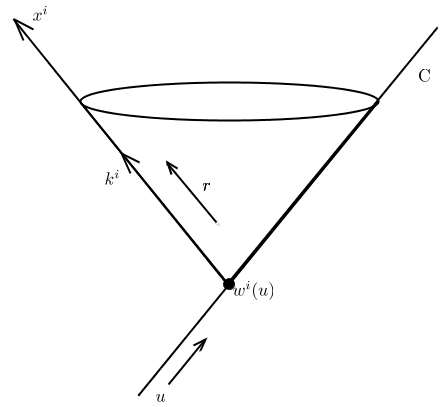
\includegraphics[scale=0.8]{figs/2_1.png}
\end{center}
\end{figure}

The position vector of a point in Minkowskian space time can be written in the form

\begin{eqnarray*}
x^i - w^i (u) = r k^i, \\
\text{or } x^i = w^i(u) + r k^i. 
\end{eqnarray*}

\noindent Thus $r$ is a new parameter which tell us the shortest distance between $C$ and some point $x^i$, and $k^i$ is the unit vector in that direction, see Fig.(\ref{Reparameterization_Figure_Unit_Vector}). As $k^i$ is a unit vector it satisfies the relations

\begin{gather}
k^i k_i = 0 \label{k_rel_1},\\
k^i v_i = -1 \label{k_rel_2}.
\end{gather}

\noindent Thus $k^i$ is normalized so that $k^i$ and $v^i$ are both future pointing (HOW DOES THIS MAKE THEM BOTH FUTURE POINTING?). Making the parameterisation

\begin{gather*}
k^i = (\xi, \eta, A, B), \\
k_i = (\xi, \eta, A, -B).
\end{gather*}

\noindent We can choose any variable for the first two slots of $k^i$ so we choose $\xi$ and $\eta$ from before for convenience. Using the relation (\ref{k_rel_1}) it is clear that

\begin{equation*}
\xi^2 + \eta^2 + A^2 - B^2 = 0,
\end{equation*}

\noindent and using the relation (\ref{k_rel_2}) it is found that

\begin{gather}
A - B = -1 \label{sim_rel_1},\\
\Rightarrow A^2 - B^2 = (A + B)(A - B) = - (A + B).
\end{gather}

\noindent Which implies

\begin{equation}\label{sim_rel_2}
\xi^2 + \eta^2 = A + B. 
\end{equation}

\noindent So expressions for $A$ and $B$ are found using Eqn.(\ref{sim_rel_1}) and Eqn.(\ref{sim_rel_2}):

\begin{eqnarray*}
A = \frac{1}{2} (-1 + \xi^2 + \eta^2) \\
B = \frac{1}{2} (1 + \xi^2 + \eta^2) \\
\end{eqnarray*}

In summary so far we have

\begin{align}
x^i & = w^i (u) + r k^i \label{rel_for_trans_1},\\
w^i & = (0,0, u,u) \label{rel_for_trans_2},\\
k^i & = (\xi, \eta, \frac{1}{2} (-1 + \xi^2 + \eta^2), \frac{1}{2} (1 + \xi^2 + \eta^2)) \label{rel_for_trans_3},\\
x^i & = (x, y, z, t) \label{rel_for_trans_4}.  
\end{align}

Consider Eqn.(\ref{rel_for_trans_1}) as a coordinate transformation from $(x,y,z,t)$ to $(\xi,\eta, r, u )$ such that

\begin{align}
x & = r \xi, \nonumber \\
y & = r \eta, \nonumber \\
z & = u + \frac{r}{2} (-1 + \xi^2 + \eta^2), \nonumber \\
t & = u + \frac{r}{2} (1 + \xi^2 + \eta^2),  \label{trans_x_to_xi} 
\end{align} 

\noindent which is clear from Eqns.(\ref{rel_for_trans_1}) - (\ref{rel_for_trans_4}). Now this is applied to the Minkowskian line element of Eqn.(\ref{Kasner_after_limit_no_k}). First, the $x$ and $y$ differentials are

\begin{eqnarray*} 
dx = r \mathrm{d}\xi + \xi \mathrm{d}r, \\
\mathrm{d}y = r \mathrm{d}\eta + \eta \mathrm{d}r. 
\end{eqnarray*} 

\noindent Which gives

\begin{equation}\label{differentials_1}
{\mathrm{d}x}^2 + {\mathrm{d}y}^2 = r^2 ({\mathrm{d}\xi}^2 + {\mathrm{d}\eta}^2) + 2 r \xi {\mathrm{d}\xi} {\mathrm{d}r} + 2 r \eta {\mathrm{d}\eta}{\mathrm{d}r} + (\xi^2 + \eta^2) {\mathrm{d}r}^2.
\end{equation}

\noindent Next, the $z$ and $t$ differentials

\begin{align*}
z + t & = 2 u + r (\xi^2 + \eta^2), \\
z - t & = - r, \\
{\mathrm{d}z} + {\mathrm{d}t} & = 2 \mathrm{d}u + (\xi^2 + \eta^2) \mathrm{d}r + 2 r \xi {\mathrm{d}\xi} + 2 r \eta {\mathrm{d}\eta}, \\
{\mathrm{d}z} - {\mathrm{d}t} & = - \mathrm{d}r. 
\end{align*}

\noindent Then using difference of two squares to obtain

\begin{equation}\label{differentials_2}
{\mathrm{d}z}^2 - {\mathrm{d}t}^2 = -2 {\mathrm{d}u}{\mathrm{d}r} - (\xi^2 + \eta^2) {\mathrm{d}r}^2 - 2 r \xi {\mathrm{d}\xi}{\mathrm{d}r} - 2 r \eta {\mathrm{d}\eta}{\mathrm{d}r}.
\end{equation}

\noindent Combining Eqn.(\ref{differentials_1}) and (\ref{differentials_2}) to get:

\begin{equation*}
{\mathrm{d}x}^2 + {\mathrm{d}y}^2 + {\mathrm{d}z}^2 - {\mathrm{d}t}^2 = r^2 ({\mathrm{d}\xi}^2 + {\mathrm{d}\eta}^2) - 2 {\mathrm{d}u}{\mathrm{d}r}
\end{equation*}

\noindent and from this it is clear that Eqn.(\ref{Kasner_after_limit_no_k}) is the line element of Minkowskian space-time with $r = 0$ a null geodesic with affine parameter $u$ along it as stated at the beginning of the section.(ERROR. REFER TO GEODESIC CALC FROM EARLIER)

Thus it has been shown that the Kasner solution to the vacuum filed equations can be obtained from the Schwarzschild solution of the vacuum field equations by taking the special case where the mass goes to infinity. (ERROR. ISNT THIS A CONTRADICTION???) Then the Minkowskian space-time line element in a particular set of coordinates $(\xi, \eta, r, u)$, can be derived from the Kasner solution by setting the mass to zero. It has been shown that the special case where $r=0$ in this Minkowskian space-time is then a null geodesic with $u$ an affine parameter along it.  
